\chapter{Implementation \& Experimental Design}
\label{chap:experimental-design}

So far in this thesis we have seen examples of what a system that implements trace assisted caching might look like from a very high level. For the purposes of context, our ambition for this experiment is to design the hardware that would be necessary to implement trace assisted caching. To then evaluate the efficacy of the design we will then synthesise this design so that it can be realised inside the Xilinx VC707 \gls{fpga} \cite{UG885VC707Evaluation2019}. We will then perform measurements on the newly designed hardware, as well as on other simpler designs to attempt to demonstrate the performance increase that is seen as a result of trace-assisted caching. 

In this chapter we are going to explore the actual implementation of this scheme that was undertaken as part of this project. We'll first explore some of the pre-existing components that were used, and then follow that by discussing the development of each of the new elements that were necessary to implement the scheme. To conclude we'll discuss the actual experiment that is to be run and illustrate some of the tooling that was developed to enable this to proceed smoothly.

\section{Pre-existing Components}

When beginning the construction of the hardware necessary to implement trace-assisted caching there are several modules that we can simply re-purpose from other projects. Starting with the processor as a whole, for these experiments we are going to use the \texttt{RI5CY}\cite{gautschiNearThresholdRISCVCore2017} processor from the PULP Foundation which implements the \texttt{RISC-V} ISA. The \texttt{RI5CY} is a 32-bit, in order processor with a 4-stage pipeline. It supports the RV32I,RV32C and RV32M standards found within the \texttt{RISC-V} standard which allows for integer computation, compressed instructions and integer multiplication and division. There is an optional floating point module but that will not be included in our instance of the \texttt{RI5CY} because it simplifies tracking the computation of the instructions. A big benefit of the \texttt{RI5CY} is that it has a Harvard Architecture, making it ideal for these experiments because we can isolate the data memory to more accurately to quantify the benefit from trace assisted caching. In addition because the \texttt{RISC-V} ISA is based on classic \gls{risc} we don't have to be concerned about multiple esoteric addressing modes or microcode as we might have to with a \gls{cisc} architecture. To be precise only \texttt{LOAD} and \texttt{STORE} are allowed to access memory which simplifies the task of tracking memory operations significantly.

As the \texttt{RI5CY} processor is released under the OpenHardware \cite{OpenSourceHardware} initiative all of the source code is publicly available to be scrutinised and adapted if necessary. We will need to make certain changes to the \texttt{RI5CY} processor to expose some internal signals, but because we have source code access, and because Xilinx's Vivado Design Suite can synthesise this code into a hardware description for an \gls{fpga} this is relatively straightforward. This will be dealt with more fully in the next section where we discuss the trace recorder. A further benefit of using the \texttt{RI5CY} processor is that it has already been integrated into the PULPino \cite{traberPULPinoDatasheet2017} \gls{soc} which was built using the Xilinx Vivado toolchain. This means there are several ancillary hardware blocks, available online, that allow the \texttt{RI5CY}'s native memory protocol to talk to the Xilinx \texttt{AXI} protocol, used to communicate easily with the various hardware blocks on the \gls{fpga} this means we can re-use lots of different \texttt{AXI} based memory implementations without having to write our own adapter. This adapter is known as a \texttt{core2axi} block. 

Another important factor is the memory technology we will use to support the processor. Xilinx provide a feature as part of newer versions of Vivado known as \glspl{xpm}\cite{UG974UltraScaleArchitecture2018}. What these \glspl{xpm} allow is for you to specify the parameters of your memory implementation (size, address width, latency etc.) and then delegate the problem of constructing such a memory system to Vivado's in-built tool set. As memory system design can be one of the more complex areas of design when dealing with \glspl{fpga} and is not something we are that interested in for these experiments it makes sense to make use of this facility rather than manually crafting our own memory implementation. You can communicate with this memory system using the \texttt{AXI} protocol\cite{AMBAAXIACE2013}, all the interfaces for which are generated by Vivado itself. This allows us to specify the instruction memory and data memory separately in a much simpler way than having to write all the code to implement the \texttt{AXI} protocol and manage individual physical memory elements. 

So at this point we have a fully functioning processor, connected to two physically separate memory implementations, generated by the \glspl{xpm}. Between the processor and the \texttt{AXI} ports on the \gls{xpm} generated memory are two \texttt{core2axi} blocks that convert the processors native memory protocol to a set of signals that conform to the \texttt{AXI4} standard. A diagram of the current architecture can be seen in Figure \ref{fig:kuuga-architecture}.

\begin{figure}[htbp]
	\tikzstyle{block} = [draw, rectangle, text width=2cm, text centered, minimum height=2cm, node distance=2.7cm]
\tikzstyle{computation-block} = [block, fill=blue!30]
\tikzstyle{memory-block} = [block, fill=green!30]
\tikzstyle{cache-block} = [block, fill=orange!30, minimum height=1cm]

\begin{center}
	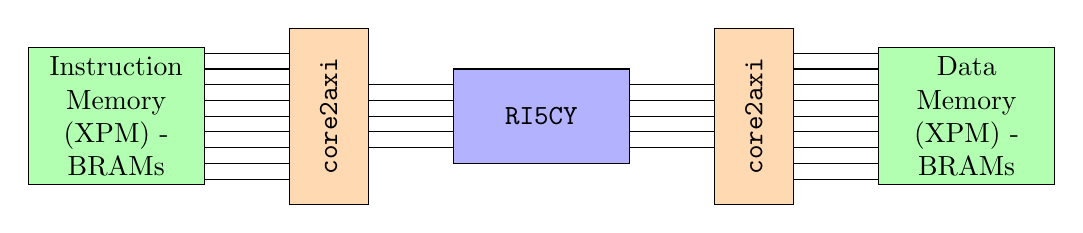
\begin{tikzpicture}
	
	 \node [computation-block] (CPU) {\texttt{RI5CY}};
	 \node [cache-block, right of=CPU, rotate=90] (core2axi-data) {\texttt{core2axi}};
	 \node [cache-block, left of=CPU, rotate=90] (core2axi-inst) {\texttt{core2axi}};
	 \node [memory-block, left of=core2axi-inst] (Imem) {Instruction Memory (XPM) - BRAMs};
	 \node [memory-block, right of=core2axi-data] (Dmem) {Data Memory (XPM) - BRAMs};
	
	\foreach \i in {-2,...,2}{% 
		\draw[-] ([yshift=\i * 0.2 cm]CPU.east) -- ([yshift=\i * 0.2 cm]core2axi-data.north) ;}
	
	\foreach \i in {-2,...,2}{% 
		\draw[-] ([yshift=\i * 0.2 cm]CPU.west) -- ([yshift=\i * 0.2 cm]core2axi-inst.south) ;}
	
	\foreach \i in {-4,...,4}{% 
		\draw[-] ([yshift=\i * 0.2 cm]core2axi-inst.north) -- ([yshift=\i * 0.2 cm]Imem.east) ;}
	
	\foreach \i in {-4,...,4}{% 
		\draw[-] ([yshift=\i * 0.2 cm]core2axi-data.south) -- ([yshift=\i * 0.2 cm]Dmem.west) ;}
	
	\end{tikzpicture}
\end{center}
	\caption[The Basic Implemented Architecture]{The resulting architecture that is used as a starting point for implementing the more complex parts of trace-assisted caching. The Memory protocols used are the \texttt{RI5CY}'s built in protocol before the \texttt{core2axi} adapter where the protocol is converted to \texttt{AXI4} for communication with the \glspl{xpm}. The \glspl{xpm} are implemented as collections of \glspl{bram}}
	\label{fig:kuuga-architecture}
\end{figure}

\section{Trace Recorder (Gouram)}

Now that we have a starting point it's possible to consider the construction of the trace recorder part of Kuuga, this will be known as Gouram. To start with, we need a way to track the execution of each instruction as it passes through the various pipeline stages of the processor. Further to that we need to track the effective addresses of each memory instruction as they are generated by the running program. The basic construction for this new piece of hardware will be to have it made of two sub-modules, the first will track the \texttt{IF}/\texttt{ID} phase of the pipeline execution and the second will track the \texttt{EX} phase. We do not need to track the \texttt{WB} phase because it will have no bearing on either the effective address or the timing of other instructions as it's merely a formality that results get written back to registers. This overall architecture can be seen in Figure \ref{fig:gouram-architecture}. First to help us understand how each phase will work it's important that we understand the memory protocol that is implemented by the \texttt{RI5CY} processor. With that in hand we can move forward to describing each of sub-blocks and then the overall trace recorder module and the data it produces.

\begin{figure}
	\tikzstyle{block} = [draw, rectangle, text width=2cm, text centered, minimum height=1.2cm, node distance=2.7cm,fill=blue!30]
\tikzstyle{container} = [draw, rectangle, inner sep=0.3cm, fill=orange!50,minimum height=3cm, minimum width=3cm]
\def\bottom#1#2{\hbox{\vbox to #1{\vfill\hbox{#2}}}}
\tikzset{
	mybackground/.style={execute at end picture={
			\begin{scope}[on background layer]
				\node[] at (current bounding box.north){\bottom{1cm} #1};
			\end{scope}
	}},
}

\begin{center}
	\begin{tikzpicture}
	
	\node [block,  minimum height=3cm] (if-tracker) {\texttt{IF} Tracker};
	\node [block, below of=if-tracker] (counter) {Monotonic Counter};
	\node [block, right=1.5cm and 1cm of if-tracker, minimum height=4.5cm, yshift=-0.9cm] (ex-tracker) {\texttt{EX} Tracker};
	\begin{scope}[on background layer]
	\node [container,fit=(if-tracker) (counter) (ex-tracker),label=above:Gouram] (container) {};
	\end{scope}
	
	\foreach \i in {-6,...,6}{% 
		\draw[-] ([yshift=\i * 0.3 cm, xshift=-1cm]container.west) -- ([yshift=\i * 0.3cm]container.west);
	}

	\foreach \i in {-3,...,3}{% 
	\draw[-] ([yshift=\i * 0.3 cm]container.east) -- ([yshift=\i * 0.3cm, xshift=1cm]container.east);
		}
	
	\draw [decorate,decoration={brace,amplitude=10pt,raise=4pt},yshift=0pt]
	([yshift=-1.5cm, xshift=1cm]container.north east) -- ([yshift=1.5cm, xshift=1cm]container.south east) node [black,midway,rotate=90, yshift=-1cm] {Trace Data Output};
	
	\draw [decorate,decoration={brace,amplitude=10pt,raise=4pt,mirror},yshift=0pt]
	([yshift=-0.3cm, xshift=-1cm]container.north west) -- ([yshift=0.3cm, xshift=-1cm]container.south west) node [black,midway,rotate=90, yshift=1cm] {Input signals observed from processor};
	
	\draw [->, thick] (counter.north) -- (if-tracker.south);
	
	\draw [->, thick] (counter.east) -- ([xshift=0.2cm]counter.east) |- ([yshift=-0.1cm]ex-tracker.west);
	\draw [->, thick] (if-tracker.east) -- ([xshift=0.2cm]if-tracker.east) |- ([yshift=0.1cm]ex-tracker.west);
	
	\end{tikzpicture}
\end{center}
	\caption[Gouram High Level Architecture]{The modules and connections that make up Gouram and its tracking capabilities. There are some other ancillary connections that are omitted from this diagram including the clock and reset lines for each module. These are omitted to add clarity to the diagram.}
	\label{fig:gouram-architecture}
\end{figure}

\subsection{\texttt{RI5CY} Memory Protocol}

The memory protocol that is implemented by the \texttt{RI5CY} is documented in the processor manual \cite{andreastraberRI5CYUserManual2017}. However it bears slightly further explanation there are certain parts of the protocol that we will rely on or have to workaround in order for Gouram to function correctly. To begin there are 8 signals that the \gls{lsu} uses to communicate with the memory hardware and these are listed in the Figure \ref{fig:signal-table}, reproduced from the processor manual:

\begin{figure}[htbp]
	\renewcommand{\arraystretch}{1.4}
	\begin{tabular}{lccp{7cm}}
		\hline
		\textbf{Signal} & \textbf{Bit Width} &\textbf{Direction} & \textbf{Description} \\
		\hline
		\texttt{data\_req\_o}
& 1 & Output & Request ready, must stay high until \texttt{data\_gnt\_i} is high for one cycle. \\
		\texttt{data\_addr\_o} & 32 & Output & Address \\
	  	\texttt{data\_we\_o}
& 1 & Output & Write Enable, high for writes, low for reads. Sent together with \texttt{data\_req\_o}. \\
	  	\texttt{data\_be\_o} & 4 & Output & Byte Enable. Is set for the bytes to write/read, sent together with \texttt{data\_req\_o}. \\
	  	\texttt{data\_wdata\_o} & 32
& Output & Data to be written to memory, sent together with \texttt{data\_req\_o}. \\
	  	\texttt{data\_rdata\_i} & 32 & Input & Data read from memory. \\
		\texttt{data\_rvalid\_i} & 1 & Input & \texttt{data\_rdata\_i} holds valid data when \texttt{data\_rvalid\_i} is high. This signal will be high for exactly one cycle per request. \\
		\texttt{data\_gnt\_i} & 1 & Input & The other side accepted the request. \texttt{data\_addr\_o} may change in the next cycle. \\
		\hline
	\end{tabular}
\caption{List of input and output signals provided by the \gls{lsu} to implement the memory protocol for the \texttt{RI5CY}, reproduced from the processor manual \cite{andreastraberRI5CYUserManual2017}}
\label{fig:signal-table}
\end{figure}

The protocol then proceeds thus. When an instruction requires access to memory the \gls{lsu} sets \texttt{data\_req\_o} high, whilst at the same time placing the calculated address (\texttt{data\_addr\_o}, byte enable bits (\texttt{data\_be\_o}), any data to be written to memory (\texttt{data\_wdata\_o)} and selecting a read or a write with \texttt{data\_we\_o}. Then the processor waits for the memory system to respond by setting \texttt{data\_gnt\_i} high. Once this has happened the processor can change any of the 4 signals it set originally, assuming them to be cached in the memory controller now \texttt{data\_gnt\_i} is high. This may happen in the same cycle that \texttt{data\_req\_o} goes high or it may take several cycles with a slower memory technology. After the grant the memory system will execute the load or store as required and once it has completed it will set \texttt{data\_rvalid\_i} high. This will happen after at least 1 clock cycle from the setting of \texttt{data\_gnt\_i} to high. Once \texttt{data\_rvalid\_i} is high \texttt{data\_rdata\_i} will contain the fetched data from memory in the case of a \texttt{LOAD} or arbitrary data in the case of a \texttt{STORE}. If another memory request is queued, \texttt{data\_req\_o} will be set high at the same time that \texttt{data\_rvalid\_i} is and the processor continues. Several examples of timing diagrams are included below in Figure \ref{fig:memory-protocol} to illustrate how this protocol works.
	
\begin{figure}[htbp]
	\begin{subfigure}{\textwidth}
		\begin{center}
			\begin{tikztimingtable}[timing/xunit=30, timing/yunit=8]
				clk        			& 19{c}@{\gtikzset{timing/rowdist=3}}\\
				data\_req\_o       	& 5l3h11l\\
				data\_addr\_o		& 5u3d{0xFEEC}11u\\
				data\_be\_o			& 5u3d{0xF}11u\\
				data\_gnt\_i		& 7lh11l\\
				data\_rvalid\_i		& 11lh7l\\
				data\_rdata\_i		& 11u5d{0xAABBCCDD}3u\\
				\extracode \background
				\begin{scope}[gray,semitransparent,semithick,node font=\tiny,anchor=west]
					\vertlines{0.5,...,\twidth}
				\end{scope}
				\endbackground
			\end{tikztimingtable}
			\caption{A \texttt{LOAD} instruction to retrieve the contents of address \texttt{0xFEEC} from memory.}
\end{center}
	\end{subfigure}
	\begin{subfigure}{\textwidth}
		\begin{center}
			\begin{tikztimingtable}[timing/xunit=30, timing/yunit=8]
				clk        			& 19{c}@{\gtikzset{timing/rowdist=3}}\\
				data\_req\_o       	& 5l3h11l\\
				data\_addr\_o		& 5u3d{0xFEEC}11u\\
				data\_we\_o			& 5l3h11l\\
				data\_be\_o			& 5u3d{0xF}11u\\
				data\_wdata\_o		& 5u3d{0x4256FFCC}11u\\
				data\_gnt\_i		& 7lh11l\\
				data\_rvalid\_i		& 11lh7l\\
				\extracode \background
				\begin{scope}[gray,semitransparent,semithick,node font=\tiny,anchor=west]
					\vertlines{0.5,...,\twidth}
				\end{scope}
				\endbackground
			\end{tikztimingtable}
			\caption{A \texttt{STORE} instruction to \texttt{0xFEEC} from the processor.}
		\end{center}
	\end{subfigure}
	\begin{subfigure}{\textwidth}
		\begin{center}
		\begin{tikztimingtable}[timing/xunit=30, timing/yunit=8]
			clk        			& 19{c}@{\gtikzset{timing/rowdist=3}}\\
			data\_req\_o       	& 5l3h3l3h5l\\
			data\_addr\_o		& 5u3d{0xFEEC}3u3d{0xFFF8}5u\\
			data\_be\_o			& 5u3d{0xF}3u3d{0xF}5u\\
			data\_we\_o			& 11l3h5l\\
			data\_wdata\_o		& 11u3d{0x778899AA}5u\\
			data\_gnt\_i		& 7lh5lh5l\\
			data\_rvalid\_i		& 11lh4lh2l\\
			data\_rdata\_i		& 11u5d{0xAABBCCDD}3u\\
			\extracode \background
			\begin{scope}[gray,semitransparent,semithick,node font=\tiny,anchor=west]
				\vertlines{0.5,...,\twidth}
			\end{scope}
			\endbackground
		\end{tikztimingtable}
		\caption{A \texttt{LOAD} followed immediately by a \texttt{STORE}}
\end{center}
	\end{subfigure}
	\caption{Several examples of the signal transitions that occur when memory transactions happen. Further of these diagrams can be seen in the \texttt{RI5CY} instruction manual. It should be noted however that the diagram in the manual labelled ``back-to-back'' does not occur in our context because of the memory implementation used.}
	\label{fig:memory-protocol}
\end{figure}

It should be pointed out that this protocol works for the instruction memory as well but uses a reduced number of signals as the instruction memory cannot be written to. These signals are labelled \texttt{inst\_req\_o} etc.

\subsection{The \texttt{IF} Module}

So now that we have the memory protocol in hand we can begin to construct sub-modules to record various parts of the execution of instructions. Looking at this generically the first thing that will happen is the instruction will be fetched from the instruction memory, as we can have no idea what the instruction is going to be until it has been fetched we have no choice but to track everything fetched by the processor and to then throw out the non-memory instructions later. This leads us to defining a module called the \texttt{IF} module which will follow a pre-defined state machine. The machine and its transitions can be seen below, and by example we'll work through each of the transitions to describe its function. The SystemVerilog code that was produced for this and subsequent hardware pieces can be seen on \href{URL} GitHub.

\begin{figure}[htbp]
	\begin{subfigure}{\textwidth}
	\begin{center}
		\begin{tikzpicture} [shorten >=1pt,node distance=4cm,on grid]
		\node[state,initial] (track-req) [font=\ttfamily] {TRACK\_REQ}; 
		\node[state] (track-gnt) [right=of track-req,font=\ttfamily]{TRACK\_GNT};
		\node[state] (track-rvalid) [right=of track-gnt,font=\ttfamily]{TRACK\_RVALID}; 
		
		\path[->] (track-req)  		edge 				node [above] {A} (track-gnt);
		\path[->] (track-req)  		edge [bend left]	node [above] {B} (track-rvalid);
		\path[->] (track-gnt)  		edge [bend left]	node [below] {C} (track-rvalid);
		\path[->] (track-rvalid)  	edge [bend left]	node [below] {D} (track-req);
		\path[->] (track-rvalid)  	edge [bend left]	node [above] {E} (track-gnt);
		
		\end{tikzpicture}
		\caption{Instruction Fetch State Machine - This effectively tracks the internal state of the fetch process}
	\end{center}
\end{subfigure}
\begin{subfigure}{\textwidth}
	\begin{center}
		\begin{tikzpicture} [shorten >=1pt,node distance=4cm,on grid]
		\node[state,initial] (idle) [font=\ttfamily] {IDLE}; 
		\node[state] (check-branch) [right=of idle,font=\ttfamily]{CHECK\_BRANCH\_DEC};
		
		\path[->] (idle)  		edge [loop above]			node [above] {F} (idle);
		\path[->] (idle)  		edge [bend left]	node [above] {G} (check-branch);
		\path[->] (check-branch)  		edge [bend left]	node [above] {H} (idle);
		
		\end{tikzpicture}
	\caption{Branch Decision State Machine - This tracks if a branch decision needs to be made and acts accordingly.}
	\end{center}
\end{subfigure}
\begin{subfigure}{\textwidth}
	\begin{center}
		\begin{tikzpicture} [shorten >=1pt,node distance=4cm,on grid]
		\node[state,initial] (find-data) [font=\ttfamily] {FIND\_DATA}; 
		\node[state] (output-data) [right=of idle,font=\ttfamily]{OUTPUT\_DATA};
		
		\path[->] (find-data)  		edge [bend left]	node [above] {I} (output-data);
		\path[->] (output-data)  		edge [bend left]	node [above] {J} (find-data);
		
		\end{tikzpicture}
		\caption{Output State Machine - This uses the results from the first two state machines to output the correct data to the next phase of the process}
	\end{center}
\end{subfigure}

	\caption{The three state machines that make up the execution of the IF Module inside Gouram. These state machines all work concurrently as per the semantics of SystemVerilog.}
	\label{fig:if-state-machine}
\end{figure}

\subsubsection{Instruction Fetch State Machine}

Upon boot each of the state machines will be reset to the \texttt{IDLE} state and each clock cycle will check for the signals necessary to transition to the other states. So the first thing that will happen is the program counter will attempt to fetch the next instruction as pointed to by the program counter. This will cause the \texttt{instr\_req\_o} signal to be set high which will trigger the \texttt{IDLE} state to make a decision as to whether to take transition \texttt{A} or \texttt{B}. The RI5CY manual defines that \texttt{instr\_gnt\_i} could become high in the same clock cycle as \texttt{instr\_req\_o} so if that's the case we then need to transition to \texttt{TRACK\_RVALID} otherwise the \texttt{gnt} signal will be missed, so transition \texttt{B} is taken. Otherwise it is transition \texttt{A}. If transition \texttt{B} is taken then the instruction address and the value of monotonic counter are stored as they could change in the next clock cycle which means the information would be lost. This data is stored in a buffer that builds up the required information over time and then sets a flag to mark it as ready to be passed to the next phase.

If transition \texttt{A} is taken the state machine then waits for \texttt{instr\_gnt\_i} to go high and then captures the same information as described previously. Now in either case once we arrive in state \texttt{TRACK\_RVALID} the state machine waits for \texttt{instr\_rvalid\_i} to be set high and when that happens the instruction data is captured into the buffer along with the time at which the \texttt{instr\_rvalid\_i} went high, again from the monotonic counter. After this either transition \texttt{D} is taken to bring us back to waiting for a new \texttt{req} signal or, because it's possible for \texttt{rvalid} and \texttt{req} signals to overlap it's also possible that we might have to transition back to \texttt{TRACK\_GNT} instead and this is covered by transition \texttt{E}. 

\subsubsection{Branch Decision State Machine}

It's easy to think at this point that our job is complete and we should simply output the data now it's been captured. However the problem with this is that the instructions that are fetched could very easily be jump or branch instruction and this is not resolved until the Decode phase. Furthermore because that takes a non-trivial amount of time it's often the case that the processor will fetch instructions that are never actually executed because they are invalidated once the branch or jump has been taken. Consequently, before we decide if we can output the instruction we have just captured we have to wait for its decode phase to end and any branch conditions to be calculated. This is especially complicated by the fact that the instructions affected are the ones that occur in the window between the calculation of the jump or branch address and the successful fetch of the branch instruction. This is shown in Figure \ref{fig:weird-branch-behaviour}.

\begin{figure}[hbtp]
	\begin{center}
		\begin{tikztimingtable}[timing/xunit=15, timing/yunit=8, timing/lslope=0.1, timing/zslope=0.1, timing/dslope=0.1 ]
				counter & [timing/counter/new={char=q}] u22{q}\\
				clk        			& 45{c}\\
				instr\_req\_o       & 5l4h6l4h6l4h6l4h6l\\
				instr\_addr\_o		& 5u4d{0x27C}{[color=blue]10d{0x280}6d{0x284}}4d{0x29C}10d{0x2A0}6u\\
				instr\_gnt\_i		& 7l2h8l2h8l2h8l2h6l\\
				instr\_rvalid\_i	& 15lH8lH8lH8l\\
				instr\_rdata\_i		& 15u5D{0xF85FF0EF}{[color=blue]5D{0x00050713}}5D{0xFE442783}\\
				data\_req\_o       	& h4H18L\\
				data\_addr\_o		& d4D{0xfee4}18U\\
				data\_gnt\_i		& l3LH18L\\
				data\_rvalid\_i		& l12LH9L\\
				data\_rdata\_i		& u12U20d{0x00000005}\\
				is\_decoding		& l12LH5LH3L\\
				jump\_done			& l12LH9L\\
				\extracode \background
				\begin{scope}[gray,semitransparent,semithick,node font=\tiny,anchor=west]
					\vertlines{0.5,...,\twidth}
				\end{scope}
				\endbackground
\end{tikztimingtable}	
	\end{center}
	\caption[Branching Behaviour Edge Case]{Due to the long running data memory fetch that completes during Clock Cycle 12 the decode phase for the fetched \texttt{0xF85FF0EF}, a jump instruction does not get decoded until Clock Cycle 12. Due to the architecture of the \texttt{RI5CY} processor jump address are calculated in the Decode Phase so the decision as to whether to jump or not is not made until Clock Cycle 12 either. However, as the blue highlighted signals show, the instruction at address \texttt{0x280} has already been fetched when the decision is made to jump to address \texttt{0x29C}. 
		
	This occurs and so the next fetch is correct and the processor has a method of ignoring these incorrect fetches, this means we have to implement something similar so we don't track instructions that never happened. This example explicitly targets jump instructions but they delay is even more pronounced in branch instructions as the target address and, by proxy, branch decision are calculated in the \texttt{EX} phase.}
	\label{fig:weird-branch-behaviour}
\end{figure}

When we want to track instructions that execute while a branch condition is being calculated we work in the following way. When the decode phase is complete for a potential branching instruction the code will extract the instruction from the tracking buffer and also will test whether this instruction was granted after the last branch decision was made. For the sake of argument let us assume that is true so we are not at present in a branching state. The next operation will be to store the time at which the decode phase ended and then we will test what kind of instruction we are dealing with. This is important because there are 3 situations that here could arise:

\begin{enumerate}
	\item The instruction is not a branching or jump instruction and has not been output while the processor is in a branching state. In which case we can simply output this into the next module in the tracker.
	\item The instruction is a jump instruction in which case it will be executed immediately because the calculation of the address is done in the Decode phase for optimisation reasons.
	\item The instruction is a branching instruction so we have to wait for the end of the execution phase before we know if we have to jump.
\end{enumerate}

If we are in situation 3, we trigger the Branch Decision State Machine to take transition \texttt{G}, we also set the \texttt{branching} variable such that we now know that we're waiting for a branch decision to be made. This means that no more of the tracking buffer will be processed until we have reached a branch decision. Once that happens we store the time at which the branch decision was made, what it was and update the cut off time accordingly, we also mark the instruction as ready for output in the tracking buffer. After this transition \texttt{H} is taken to move us back to the \texttt{IDLE} state. If we had been in situation 2 something similar would have happened but it would have happened immediately after the end of the decode phase. 

\subsubsection{The Output State Machine}

As all the state machines are asynchronous except for where they explicitly synchronise the last state machine is comparatively simple. The \texttt{FIND\_DATA} state simply sits and scans through the tracking buffer to see if there are any pieces of data that can be output. If it finds one it checks to see if it's a \texttt{LOAD} or a \texttt{STORE} instruction and it also checks that it was not fetched during a period where a branch decision was pending and eventually taken. This stop the situation where the processor eagerly fetched the next seequential instruction but actually ended up branching and so executed a completely different instruction. At this point it takes transition \texttt{I} to the \texttt{OUTPUT\_DATA} state. Once in that state the data is transferred to the next module that makes up Gouram along with some other data to help find the length of the execution phase. The data is marked as having been output and then transition \texttt{J} is taken and the process begins again.

\subsection{Examples}

What is described is very complicated because tracking the behaviour of the processor as it calculates branches is highly non-trivial. The best way to explore how this works is by following two examples from end to end. The first example will be the instruction at address \texttt{0x258} in Figure \ref{fig:trace-with-original}, which is \texttt{0x00112e23}. The second will be a more complex branching example by following \texttt{0xfce7dae3} at address \texttt{0x2a4} which also appears in the same figure.

\subsubsection{Simple Load Example}

The diagram of the signals issued by the memory system can be seen in Figure \ref{fig:simple-load-signal-diagram}. We will also track the contents of the tracking buffer and the state machines so we can see how all of the aspects of this fit together. An empty entry in the tracking buffer and the state machines at the start of the execution can be seen in Figure \ref{fig:load-example-starting-state} resp. The names of the states in the machine have been shortened into acronyms for reasons of space but they are the same as the diagram in \ref{fig:if-state-machine}. 

\begin{figure}[htbp]
		\begin{center}
	\begin{tikztimingtable}[timing/xunit=30, timing/yunit=8, timing/lslope=0, timing/dslope=0.1]
		counter & [timing/counter/new={char=q}] u9{q}\\
		clk        			& 19{c}@{\gtikzset{timing/rowdist=3}}\\
		inst\_req\_o       	& 5l4h10l\\
		instr\_addr\_o		& 5u4d{0x258}10u\\
		instr\_gnt\_i		& 7l2h10l\\
		instr\_rvalid\_i		& 11l2h6l\\
		instr\_rdata\_i		& 11u8d{0x00112e23}\\
		is\_decoding		& 13lH4l\\
		id\_ready			& 13lH4l\\
		\extracode \background
		\begin{scope}[gray,semitransparent,semithick,node font=\tiny,anchor=west]
			\vertlines{0.5,...,\twidth}
		\end{scope}
		\endbackground
	\end{tikztimingtable}
\end{center}
		\caption{Fetching the instruction \texttt{0x00112e23} from memory}
		\label{fig:simple-load-signal-diagram}
\end{figure}

\begin{figure}[htbp]
	\begin{subfigure}{\linewidth}
		\begin{tikzpicture}
\matrix [
space, 
column 1/.style={nodes={cell,minimum width=6em}},
column 2/.style={nodes={cell,minimum width=6em}},
column 3/.style={nodes={cell,minimum width=7em}},
column 4/.style={nodes={cell,minimum width=6em}},
column 5/.style={nodes={cell,minimum width=6em}},
column 6/.style={nodes={cell,minimum width=6em}}
] 
(tracking-buffer-1)
{
	\textbf{INST} & \textbf{ADDR} & \textbf{REQ\_START} & \textbf{GNT} & \textbf{RVALID} & \textbf{DEC\_END} \\
	\texttt{X} & \texttt{X} & \texttt{X} & \texttt{X} & \texttt{X} & \texttt{X} \\
};

\matrix [
space, below=of tracking-buffer-1,
column 1/.style={nodes={cell,minimum width=9em}},
column 2/.style={nodes={cell,minimum width=11em}},
column 3/.style={nodes={cell,minimum width=9em}},
column 4/.style={nodes={cell,minimum width=7em}}
] 
(tracking-buffer-1)
{
	\textbf{BRANCH\_DEC} & \textbf{BRANCH\_DEC\_TIME} & \textbf{OUTPUT\_READY} & \textbf{FINISHED} \\
	\texttt{X} & \texttt{X} & \texttt{0} & \texttt{0} \\
};
\end{tikzpicture}
		\caption{Schematic of a single record in the tracking buffer that will be filled out as this example progresses.}
	\end{subfigure}
	\begin{subfigure}{\linewidth}
		\begin{center}
	\begin{tikzpicture} [shorten >=1pt,node distance=3cm,on grid]
	\node[state,initial] (track-req) [font=\ttfamily, fill=blue!30] {TR}; 
	\node[state] (track-gnt) [right=of track-req,font=\ttfamily]{TG};
	\node[state] (track-rvalid) [right=of track-gnt,font=\ttfamily]{TRV}; 
	
	\path[->] (track-req)  		edge 				node [above] {A} (track-gnt);
	\path[->] (track-req)  		edge [bend left]	node [above] {B} (track-rvalid);
	\path[->] (track-gnt)  		edge [bend left]	node [below] {C} (track-rvalid);
	\path[->] (track-rvalid)  	edge [bend left]	node [below] {D} (track-req);
	\path[->] (track-rvalid)  	edge [bend left]	node [above] {E} (track-gnt);
	
	\node[state,initial] (find-data) [font=\ttfamily, right=of track-rvalid, fill=blue!30] {FD}; 
	\node[state] (output-data) [right=of find-data,font=\ttfamily]{OD};
	
	\path[->] (find-data)  		edge [bend left]	node [above] {I} (output-data);
	\path[->] (output-data)  		edge [bend left]	node [above] {J} (find-data);
	
	\end{tikzpicture}
\end{center}

		\caption{A reduced version of the previously described state machines to allow us to follow the progress of the hardware as we progress through the example. The light blue highlight indicates the current state of the machine, with the Output State}
	\end{subfigure}
\caption{The state of the \texttt{IF} tracker, we'll return to updated versions of these diagrams as we progress through the example}
\label{fig:load-example-starting-state}
\end{figure}

The process begins as \texttt{instr\_req\_o} goes high at Clock Cycle 2 and this will cause the Instruction Fetch State Machine to take transition \texttt{A} to the \texttt{TRACK\_GNT} phase. In doing so the tracking buffer will have its entry cleared out. This is necessary because it's a circular buffer so there could be data left over from a previous instruction. Then the value of the counter will be stored at the start of the \texttt{instr\_req}, this can be seen in Figure \ref{fig:load-example-step-1}. 

\begin{figure}[htbp]
	\begin{subfigure}{\linewidth}
		\begin{tikzpicture}
\matrix [
space, 
column 1/.style={nodes={cell,minimum width=6em}},
column 2/.style={nodes={cell,minimum width=6em}},
column 3/.style={nodes={cell,minimum width=7em}},
column 4/.style={nodes={cell,minimum width=6em}},
column 5/.style={nodes={cell,minimum width=6em}},
column 6/.style={nodes={cell,minimum width=6em}}
] 
(tracking-buffer-1)
{
	\textbf{INST} & \textbf{ADDR} & \textbf{REQ\_START} & \textbf{GNT} & \textbf{RVALID} & \textbf{DEC\_END} \\
	\texttt{X} & \texttt{X} & \texttt{2} & \texttt{X} & \texttt{X} & \texttt{X} \\
};

\matrix [
space, below=of tracking-buffer-1,
column 1/.style={nodes={cell,minimum width=9em}},
column 2/.style={nodes={cell,minimum width=11em}},
column 3/.style={nodes={cell,minimum width=9em}},
column 4/.style={nodes={cell,minimum width=7em}}
] 
(tracking-buffer-1)
{
	\textbf{BRANCH\_DEC} & \textbf{BRANCH\_DEC\_TIME} & \textbf{OUTPUT\_READY} & \textbf{FINISHED} \\
	\texttt{X} & \texttt{X} & \texttt{0} & \texttt{0} \\
};
\end{tikzpicture}
	\end{subfigure}
	\begin{subfigure}{\linewidth}
		\begin{center}
	\begin{tikzpicture} [shorten >=1pt,node distance=3cm,on grid]
	\node[state,initial] (track-req) [font=\ttfamily] {TR}; 
	\node[state] (track-gnt) [right=of track-req,font=\ttfamily, fill=blue!30]{TG};
	\node[state] (track-rvalid) [right=of track-gnt,font=\ttfamily]{TRV}; 
	
	\path[->] (track-req)  		edge 				node [above] {A} (track-gnt);
	\path[->] (track-req)  		edge [bend left]	node [above] {B} (track-rvalid);
	\path[->] (track-gnt)  		edge [bend left]	node [below] {C} (track-rvalid);
	\path[->] (track-rvalid)  	edge [bend left]	node [below] {D} (track-req);
	\path[->] (track-rvalid)  	edge [bend left]	node [above] {E} (track-gnt);
	
	\node[state,initial] (find-data) [font=\ttfamily, below=of track-rvalid, fill=blue!30] {FD}; 
	\node[state] (output-data) [right=of find-data,font=\ttfamily]{OD};
	
	\path[->] (find-data)  		edge [bend left]	node [above] {I} (output-data);
	\path[->] (output-data)  		edge [bend left]	node [above] {J} (find-data);
	
	\end{tikzpicture}
\end{center}

	\end{subfigure}
	\caption{}
	\label{fig:load-example-step-1}
\end{figure}


Then the grant phase will continue until clock cycle 3 when \texttt{instr\_gnt\_i} goes high. This will cause the tracking buffer to be updated with the instructions address and the time at which the \texttt{instr\_gnt\_i} went high and cause transition \texttt{C} to be taken. Then at Clock Cycle 5 \texttt{TRACK\_RVALID} will store the final pieces in the tracking buffer. The net result of these two steps can be seen in Figure \ref{fig:load-example-step-2}. Following this transition \texttt{D} will be taken back to \texttt{TRACK\_REQ} to track the next instruction.

\begin{figure}[htbp]
	\begin{subfigure}{\linewidth}
		\begin{tikzpicture}
\matrix [
space, 
column 1/.style={nodes={cell,minimum width=6em}},
column 2/.style={nodes={cell,minimum width=6em}},
column 3/.style={nodes={cell,minimum width=7em}},
column 4/.style={nodes={cell,minimum width=6em}},
column 5/.style={nodes={cell,minimum width=6em}},
column 6/.style={nodes={cell,minimum width=6em}}
] 
(tracking-buffer-1)
{
	\textbf{INST} & \textbf{ADDR} & \textbf{REQ\_START} & \textbf{GNT} & \textbf{RVALID} & \textbf{DEC\_END} \\
	\texttt{0x00112e23} & \texttt{0x258} & \texttt{2} & \texttt{3} & \texttt{5} & \texttt{X} \\
};

\matrix [
space, below=of tracking-buffer-1,
column 1/.style={nodes={cell,minimum width=9em}},
column 2/.style={nodes={cell,minimum width=11em}},
column 3/.style={nodes={cell,minimum width=9em}},
column 4/.style={nodes={cell,minimum width=7em}}
] 
(tracking-buffer-1)
{
	\textbf{BRANCH\_DEC} & \textbf{BRANCH\_DEC\_TIME} & \textbf{OUTPUT\_READY} & \textbf{FINISHED} \\
	\texttt{X} & \texttt{X} & \texttt{0} & \texttt{0} \\
};
\end{tikzpicture}
	\end{subfigure}
	\begin{subfigure}{\linewidth}
		\begin{center}
	\begin{tikzpicture} [shorten >=1pt,node distance=3cm,on grid]
	\node[state,initial] (track-req) [font=\ttfamily] {TR}; 
	\node[state] (track-gnt) [right=of track-req,font=\ttfamily]{TG};
	\node[state] (track-rvalid) [right=of track-gnt,font=\ttfamily, fill=blue!30]{TRV}; 
	
	\path[->] (track-req)  		edge 				node [above] {A} (track-gnt);
	\path[->] (track-req)  		edge [bend left]	node [above] {B} (track-rvalid);
	\path[->] (track-gnt)  		edge [bend left]	node [below] {C} (track-rvalid);
	\path[->] (track-rvalid)  	edge [bend left]	node [below] {D} (track-req);
	\path[->] (track-rvalid)  	edge [bend left]	node [above] {E} (track-gnt);
	
	\node[state,initial] (find-data) [font=\ttfamily, right=of track-rvalid, fill=blue!30] {FD}; 
	\node[state] (output-data) [right=of find-data,font=\ttfamily]{OD};
	
	\path[->] (find-data)  		edge [bend left]	node [above] {I} (output-data);
	\path[->] (output-data)  		edge [bend left]	node [above] {J} (find-data);
	
	\end{tikzpicture}
\end{center}

	\end{subfigure}
	\caption{}
	\label{fig:load-example-step-2}
\end{figure}

Once the decode phase of this instruction is complete, the processor signals this by setting the internal signals \texttt{is\_decoding} and \texttt{id\_ready} high in clock cycle 6. At this point the tracking buffer will be linearly scanned and the entry generated for \texttt{0x00112e23} will be marked as the earliest unprocessed index. Since we haven't yet encountered a branch or jump instruction we are not in a pending branching state which means we can store we are in situation 1 as above. Consequently we store the end of the decode phase and then mark this instruction as ready for output. 

\begin{figure}[htbp]
	\begin{tikzpicture}
\matrix [
space, 
column 1/.style={nodes={cell,minimum width=6em}},
column 2/.style={nodes={cell,minimum width=6em}},
column 3/.style={nodes={cell,minimum width=7em}},
column 4/.style={nodes={cell,minimum width=6em}},
column 5/.style={nodes={cell,minimum width=6em}},
column 6/.style={nodes={cell,minimum width=6em}}
] 
(tracking-buffer-1)
{
	\textbf{INST} & \textbf{ADDR} & \textbf{REQ\_START} & \textbf{GNT} & \textbf{RVALID} & \textbf{DEC\_END} \\
	\texttt{0x00112e23} & \texttt{0x258} & \texttt{2} & \texttt{3} & \texttt{5} & \texttt{6} \\
};

\matrix [
space, below=of tracking-buffer-1,
column 1/.style={nodes={cell,minimum width=9em}},
column 2/.style={nodes={cell,minimum width=11em}},
column 3/.style={nodes={cell,minimum width=9em}},
column 4/.style={nodes={cell,minimum width=7em}}
] 
(tracking-buffer-1)
{
	\textbf{BRANCH\_DEC} & \textbf{BRANCH\_DEC\_TIME} & \textbf{OUTPUT\_READY} & \textbf{FINISHED} \\
	\texttt{X} & \texttt{X} & \texttt{1} & \texttt{0} \\
};
\end{tikzpicture}
	\caption{}
	\label{fig:load-example-step-3}
\end{figure}

In the next clock cycle the Output State Machine will scan the tracking buffer until it finds data that is marked ready for output (it additionally checks some other conditions but we will omit these for now). It will find the data for \texttt{0x00112e23}, and run a simple check to ensure this is a \texttt{LOAD}/\texttt{STORE} instruction by looking at its opcode and so will take transition \texttt{I} to the \texttt{OUTPUT\_DATA} state where it will transfer the data into the next module. Following that it will mark \texttt{0x00112e23} as finished and then transition back via \texttt{J} to the \texttt{FIND\_DATA} state. This can be seen in Figure \ref{fig:load-example-step-4}.

\begin{figure}[htbp]
	\begin{subfigure}{\linewidth}
		\begin{tikzpicture}
\matrix [
space, 
column 1/.style={nodes={cell,minimum width=6em}},
column 2/.style={nodes={cell,minimum width=6em}},
column 3/.style={nodes={cell,minimum width=7em}},
column 4/.style={nodes={cell,minimum width=6em}},
column 5/.style={nodes={cell,minimum width=6em}},
column 6/.style={nodes={cell,minimum width=6em}}
] 
(tracking-buffer-1)
{
	\textbf{INST} & \textbf{ADDR} & \textbf{REQ\_START} & \textbf{GNT} & \textbf{RVALID} & \textbf{DEC\_END} \\
	\texttt{0x00112e23} & \texttt{0x258} & \texttt{2} & \texttt{3} & \texttt{5} & \texttt{6} \\
};

\matrix [
space, below=of tracking-buffer-1,
column 1/.style={nodes={cell,minimum width=9em}},
column 2/.style={nodes={cell,minimum width=11em}},
column 3/.style={nodes={cell,minimum width=9em}},
column 4/.style={nodes={cell,minimum width=7em}}
] 
(tracking-buffer-1)
{
	\textbf{BRANCH\_DEC} & \textbf{BRANCH\_DEC\_TIME} & \textbf{OUTPUT\_READY} & \textbf{FINISHED} \\
	\texttt{X} & \texttt{X} & \texttt{1} & \texttt{1} \\
};
\end{tikzpicture}
	\end{subfigure}
	\begin{subfigure}{\linewidth}
		\begin{center}
	\begin{tikzpicture} [shorten >=1pt,node distance=3cm,on grid]
	\node[state,initial] (track-req) [font=\ttfamily, fill=blue!30] {TR}; 
	\node[state] (track-gnt) [right=of track-req,font=\ttfamily]{TG};
	\node[state] (track-rvalid) [right=of track-gnt,font=\ttfamily]{TRV}; 
	
	\path[->] (track-req)  		edge 				node [above] {A} (track-gnt);
	\path[->] (track-req)  		edge [bend left]	node [above] {B} (track-rvalid);
	\path[->] (track-gnt)  		edge [bend left]	node [below] {C} (track-rvalid);
	\path[->] (track-rvalid)  	edge [bend left]	node [below] {D} (track-req);
	\path[->] (track-rvalid)  	edge [bend left]	node [above] {E} (track-gnt);
	
	\node[state,initial] (find-data) [font=\ttfamily, right=of track-rvalid] {FD}; 
	\node[state] (output-data) [right=of find-data,font=\ttfamily, fill=blue!30]{OD};
	
	\path[->] (find-data)  		edge [bend left]	node [above] {I} (output-data);
	\path[->] (output-data)  		edge [bend left]	node [above] {J} (find-data);
	
	\end{tikzpicture}
\end{center}

	\end{subfigure}
	\caption{}
	\label{fig:load-example-step-4}
\end{figure}

\subsubsection{Complex Branching Example}

The previous example is relatively simple but introducing branching causes several other factors to have to be taken into account. For this example we will use the signal diagram in Figure \ref{fig:complex-example-signal-diagram}. An important point to note about this diagram is that a fetch from data memory is already in progress when this diagram starts, this prevents the decode phase for \texttt{0x2A4} starting as soon as it is fetched and sets this train of events in motion.

\begin{sidewaysfigure}[htbp]
	\begin{tikztimingtable}[timing/xunit=25, timing/yunit=8, timing/lslope=0.1, timing/zslope=0.1, timing/dslope=0.1 ]
				counter & [timing/counter/new={char=q, min value=100}] u20{q}\\
				clk        			& 41{c}\\
				instr\_req\_o       & 5l4h6l4h6l4h6l4h2l\\
				instr\_addr\_o		& 5u4d{0x2A4}10d{0x2A8}8d{0x2AC}2d{0x278}10d{0x27C}2u\\
				instr\_gnt\_i		& 7l2h8l2h8l2h8l2h2l\\
				instr\_rvalid\_i	& 15lH8lH8lH4l\\
				instr\_rdata\_i		& 15u5D{0xFCE7DAE3}5D{0xFE842783}3D{0xFEC42503}\\
				data\_req\_o       	& h4H16L\\
				data\_addr\_o		& d4D{0xfee4}16U\\
				data\_gnt\_i		& l3LH16L\\
				data\_rvalid\_i		& l12LH7L\\
				data\_rdata\_i		& u12U16d{0x00000005}\\
				is\_decoding		& l12LH5LHL\\
				id\_ready			& l12LH5LHL\\
				branch\_decision	& l13LH5L\\
				\extracode \background
				\begin{scope}[gray,semitransparent,semithick,node font=\tiny,anchor=west]
					\vertlines{0.5,...,\twidth}
				\end{scope}
				\endbackground
\end{tikztimingtable}
	\caption{}
	\label{fig:complex-example-signal-diagram}
\end{sidewaysfigure}

The dynamics of Instruction Fetch State Machine are quite similar, however the big change occurs when the decode phase ends for \texttt{0xFCE7DAE3}. At the start it proceeds very much as before, \texttt{0xFCE7DAE3} is identified by the module as the earliest unprocessed instruction and we are not currently branching so we mark the end of the decode phase but then we detect \texttt{0xFCE7DAE3} as a branching instruction. So we set the \texttt{branch\_pointer} to mark this instruction as the object of the branching behaviour and then trigger the Branch Decision State Machine to take transition \texttt{G}. The net result of this can be seen in Figure \ref{fig:complex-example-step-1}.

\begin{figure}[htbp]
	\begin{subfigure}{\linewidth}
		\begin{tikzpicture}
\matrix [
space, 
column 1/.style={nodes={cell,minimum width=6em}},
column 2/.style={nodes={cell,minimum width=6em}},
column 3/.style={nodes={cell,minimum width=7em}},
column 4/.style={nodes={cell,minimum width=6em}},
column 5/.style={nodes={cell,minimum width=6em}},
column 6/.style={nodes={cell,minimum width=6em}}
] 
(tracking-buffer-1)
{
	\textbf{INST} & \textbf{ADDR} & \textbf{REQ\_START} & \textbf{GNT} & \textbf{RVALID} & \textbf{DEC\_END} \\
	\texttt{0xFCE7DAE3} & \texttt{0x2A4} & \texttt{2} & \texttt{3} & \texttt{7} & \texttt{12} \\
};

\matrix [
space, below=of tracking-buffer-1,
column 1/.style={nodes={cell,minimum width=9em}},
column 2/.style={nodes={cell,minimum width=11em}},
column 3/.style={nodes={cell,minimum width=9em}},
column 4/.style={nodes={cell,minimum width=7em}}
] 
(tracking-buffer-1)
{
	\textbf{BRANCH\_DEC} & \textbf{BRANCH\_DEC\_TIME} & \textbf{OUTPUT\_READY} & \textbf{FINISHED} \\
	\texttt{X} & \texttt{X} & \texttt{0} & \texttt{0} \\
};
\end{tikzpicture}
	\end{subfigure}
	\begin{subfigure}{\linewidth}
		\begin{center}
	\begin{tikzpicture} [shorten >=1pt,node distance=3cm,on grid]
	\node[state,initial] (track-req) [font=\ttfamily, fill=blue!30] {TR}; 
	\node[state] (track-gnt) [right=of track-req,font=\ttfamily]{TG};
	\node[state] (track-rvalid) [right=of track-gnt,font=\ttfamily]{TRV}; 
	
	\path[->] (track-req)  		edge 				node [above] {A} (track-gnt);
	\path[->] (track-req)  		edge [bend left]	node [above] {B} (track-rvalid);
	\path[->] (track-gnt)  		edge [bend left]	node [below] {C} (track-rvalid);
	\path[->] (track-rvalid)  	edge [bend left]	node [below] {D} (track-req);
	\path[->] (track-rvalid)  	edge [bend left]	node [above] {E} (track-gnt);
	
	\node[state,initial] (idle) [font=\ttfamily, right = of track-rvalid, fill=blue!30] {I}; 
	\node[state] (check-branch) [right=of idle,font=\ttfamily]{CBD};
	
	\path[->] (idle)  		edge [loop above]			node [above] {F} (idle);
	\path[->] (idle)  		edge [bend left]	node [above] {G} (check-branch);
	\path[->] (check-branch)  		edge [bend left]	node [above] {H} (idle);
	
	\node[state,initial] (find-data) [font=\ttfamily, below=of track-gnt, fill=blue!30] {FD}; 
	\node[state] (output-data) [right=of find-data,font=\ttfamily]{OD};
	
	\path[->] (find-data)  		edge [bend left]	node [above] {I} (output-data);
	\path[->] (output-data)  		edge [bend left]	node [above] {J} (find-data);
	
	\end{tikzpicture}
\end{center}

	\end{subfigure}
	\caption{}
	\label{fig:complex-example-step-1}
\end{figure} 

Now, because \texttt{0xFCE7DAE3} is a branching instruction that relies on a condition it needs to enter the execution phase in order to calculate whether a branch will be taken or not. However rather than simply stalling the processor when this happens the next instruction sequentially is fetched from instruction memory, in this case \texttt{0xFE842783}. Now because of the previously mentioned fetch from data memory this fetch actually completes before a branch decision can be made, causing a new entry to enter the tracking buffer as in Figure \ref{fig:complex-example-step-2}

\begin{figure}[htbp]
	\begin{tikzpicture}
\matrix [
space, 
column 1/.style={nodes={cell,minimum width=6em}},
column 2/.style={nodes={cell,minimum width=6em}},
column 3/.style={nodes={cell,minimum width=7em}},
column 4/.style={nodes={cell,minimum width=6em}},
column 5/.style={nodes={cell,minimum width=6em}},
column 6/.style={nodes={cell,minimum width=6em}}
] 
(tracking-buffer-1)
{
	\textbf{INST} & \textbf{ADDR} & \textbf{REQ\_START} & \textbf{GNT} & \textbf{RVALID} & \textbf{DEC\_END} \\
	\texttt{0xFCE7DAE3} & \texttt{0x2A4} & \texttt{102} & \texttt{103} & \texttt{107} & \texttt{112} \\
	\texttt{0xFE842783} & \texttt{0x2A8} & \texttt{107} & \texttt{108} & \texttt{112} & \texttt{X} \\
};

\matrix [
space, below=of tracking-buffer-1,
column 1/.style={nodes={cell,minimum width=9em}},
column 2/.style={nodes={cell,minimum width=11em}},
column 3/.style={nodes={cell,minimum width=9em}},
column 4/.style={nodes={cell,minimum width=7em}}
] 
(tracking-buffer-1)
{
	\textbf{BRANCH\_DEC} & \textbf{BRANCH\_DEC\_TIME} & \textbf{OUTPUT\_READY} & \textbf{FINISHED} \\
	\texttt{X} & \texttt{X} & \texttt{0} & \texttt{0} \\
	\texttt{X} & \texttt{X} & \texttt{0} & \texttt{0} \\
};
\end{tikzpicture}
	\caption{}
	\label{fig:complex-example-step-2}
\end{figure} 


Let us assume that in this case the branch is in fact taken, so the next instruction to be executed will be \texttt{0xFEC42503} at address \texttt{0x278}. In the \texttt{CHECK\_BRANCH\_DECISION} phase, the \texttt{branch\_decision} signal goes high so we then store the time at which that occurred and set the cut off time as 112. This cut off time is important because it defines the time at which an instruction grant would need to take place after to be a valid fetch, forming a window with the lower bound set by the grant time of the branching instruction itself. We then also set a marker to state that we are in a branching state and mark the branching instruction as ready to output. The effect of these concurrent changes, both the fetch from \texttt{0x2A8} and the effect of the branch decision state machine can be seen in Figure \ref{fig:complex-example-step-3}. The Branch Decision State Machine then returns to the \texttt{IDLE} state.

\begin{figure}[htbp]
	\begin{subfigure}{\linewidth}
		\begin{tikzpicture}
\matrix [
space, 
column 1/.style={nodes={cell,minimum width=6em}},
column 2/.style={nodes={cell,minimum width=6em}},
column 3/.style={nodes={cell,minimum width=7em}},
column 4/.style={nodes={cell,minimum width=6em}},
column 5/.style={nodes={cell,minimum width=6em}},
column 6/.style={nodes={cell,minimum width=6em}}
] 
(tracking-buffer-1)
{
	\textbf{INST} & \textbf{ADDR} & \textbf{REQ\_START} & \textbf{GNT} & \textbf{RVALID} & \textbf{DEC\_END} \\
	\texttt{0xFCE7DAE3} & \texttt{0x2A4} & \texttt{102} & \texttt{103} & \texttt{107} & \texttt{112} \\
	\texttt{0xFE842783} & \texttt{0x2A8} & \texttt{107} & \texttt{108} & \texttt{112} & \texttt{X} \\
};

\matrix [
space, below=of tracking-buffer-1,
column 1/.style={nodes={cell,minimum width=9em}},
column 2/.style={nodes={cell,minimum width=11em}},
column 3/.style={nodes={cell,minimum width=9em}},
column 4/.style={nodes={cell,minimum width=7em}}
] 
(tracking-buffer-1)
{
	\textbf{BRANCH\_DEC} & \textbf{BRANCH\_DEC\_TIME} & \textbf{OUTPUT\_READY} & \textbf{FINISHED} \\
	\texttt{1} & \texttt{112} & \texttt{0} & \texttt{0} \\
	\texttt{X} & \texttt{X} & \texttt{0} & \texttt{0} \\
};
\end{tikzpicture}
	\end{subfigure}
	\begin{subfigure}{\linewidth}
		\begin{center}
	\begin{tikzpicture} [shorten >=1pt,node distance=3cm,on grid]
	\node[state,initial] (track-req) [font=\ttfamily, fill=blue!30] {TR}; 
	\node[state] (track-gnt) [right=of track-req,font=\ttfamily]{TG};
	\node[state] (track-rvalid) [right=of track-gnt,font=\ttfamily]{TRV}; 
	
	\path[->] (track-req)  		edge 				node [above] {A} (track-gnt);
	\path[->] (track-req)  		edge [bend left]	node [above] {B} (track-rvalid);
	\path[->] (track-gnt)  		edge [bend left]	node [below] {C} (track-rvalid);
	\path[->] (track-rvalid)  	edge [bend left]	node [below] {D} (track-req);
	\path[->] (track-rvalid)  	edge [bend left]	node [above] {E} (track-gnt);
	
	\node[state,initial] (idle) [font=\ttfamily, right = of track-rvalid] {I}; 
	\node[state] (check-branch) [right=of idle,font=\ttfamily, fill=blue!30]{CBD};
	
	\path[->] (idle)  		edge [loop above]			node [above] {F} (idle);
	\path[->] (idle)  		edge [bend left]	node [above] {G} (check-branch);
	\path[->] (check-branch)  		edge [bend left]	node [above] {H} (idle);
	
	\node[state,initial] (find-data) [font=\ttfamily, below=of track-gnt, fill=blue!30] {FD}; 
	\node[state] (output-data) [right=of find-data,font=\ttfamily]{OD};
	
	\path[->] (find-data)  		edge [bend left]	node [above] {I} (output-data);
	\path[->] (output-data)  		edge [bend left]	node [above] {J} (find-data);
	
	\end{tikzpicture}
\end{center}

	\end{subfigure}
	\caption{}
	\label{fig:complex-example-step-3}
\end{figure} 

Now the Output State Machine will deal with both the accumulated instructions first it will process the \texttt{0xFCE7DAE3} and this will simply be set to finished immediately as it's not a \texttt{LOAD} or \texttt{STORE} instruction. However when it reaches the next instruction after clock cycle 118. At first it will a similar process to the simple example, it will be selected as the earliest index but then, because, as can be seen in Figure \ref{fig:complex-example-signal-diagram} its grant occurs before the cut off time we were still in branching state when the fetch occurred so this fetch is invalid. Consequently we simply mark this instruction in the tracking buffer as finished, and then search again for another instruction to assign this decode phase to. The net result of this can be seen in the final contents of the tracking buffer as shown in Figure \ref{fig:complex-example-step-4}.

\begin{figure}[htbp]
	\begin{tikzpicture}
\matrix [
space, 
column 1/.style={nodes={cell,minimum width=6em}},
column 2/.style={nodes={cell,minimum width=6em}},
column 3/.style={nodes={cell,minimum width=7em}},
column 4/.style={nodes={cell,minimum width=6em}},
column 5/.style={nodes={cell,minimum width=6em}},
column 6/.style={nodes={cell,minimum width=6em}}
] 
(tracking-buffer-1)
{
	\textbf{INST} & \textbf{ADDR} & \textbf{REQ\_START} & \textbf{GNT} & \textbf{RVALID} & \textbf{DEC\_END} \\
	\texttt{0xFCE7DAE3} & \texttt{0x2A4} & \texttt{102} & \texttt{103} & \texttt{107} & \texttt{112} \\
	\texttt{0xFE842783} & \texttt{0x2A8} & \texttt{107} & \texttt{108} & \texttt{112} & \texttt{X} \\
	\texttt{0xFEC42503} & \texttt{0x278} & \texttt{112} & \texttt{113} & \texttt{117} & \texttt{118} \\
};

\matrix [
space, below=of tracking-buffer-1,
column 1/.style={nodes={cell,minimum width=9em}},
column 2/.style={nodes={cell,minimum width=11em}},
column 3/.style={nodes={cell,minimum width=9em}},
column 4/.style={nodes={cell,minimum width=7em}}
] 
(tracking-buffer-1)
{
	\textbf{BRANCH\_DEC} & \textbf{BRANCH\_DEC\_TIME} & \textbf{OUTPUT\_READY} & \textbf{FINISHED} \\
	\texttt{1} & \texttt{112} & \texttt{1} & \texttt{1} \\
	\texttt{X} & \texttt{X} & \texttt{0} & \texttt{1} \\
	\texttt{X} & \texttt{X} & \texttt{1} & \texttt{0} \\
};
\end{tikzpicture}
	\caption{}
	\label{fig:complex-example-step-4}
\end{figure} 

This mirrors what happens in the processor where instructions that are incorrectly predicted are invalidated and therefore never propagate throughout the processor. Once we reach an instruction that is beyond the calculated cut off point we are non-longer in a branching state and so can start outputting data again in a similar fashion to before.

\subsection{The \texttt{EX} Module}

Once the process has completed in the \texttt{IF} module the pertinent data is passed into the \texttt{EX} module which tracks the data memory querying part of the process. Since we have already filtered out a lot of the instructions the process in this phase is slightly simpler however since there are dependencies between instructions this module cannot act synchronously with the processor. This means there are several signal buffers that record previously seen signal values and are then queried so that the beginning and the end of the transactions can be seen. 

\begin{figure}[htbp]
	\begin{center}
		\begin{tikzpicture} [shorten >=1pt,node distance=4.5cm,on grid]
		\node[state,initial] (ex-start) [font=\ttfamily] {EX\_START}; 
		\node[state] (get-data) [right=of track-req,font=\ttfamily]{GET\_DATA};
		\node[state] (check-mem-req) [right=of get-data,font=\ttfamily]{CHECK\_MEM\_REQ}; 
		\node[state] (scan-mem-req) [above=of check-mem-req,font=\ttfamily]{SCAN\_MEM\_REQ}; 
		\node[state] (check-mem-rvalid) [right=of check-mem-req,font=\ttfamily]{CHECK\_MEM\_RVALID}; 
		\node[state] (scan-mem-rvalid) [above=of check-mem-rvalid,font=\ttfamily]{SCAN\_MEM\_RVALID}; 
		\node[state] (output-result) [below=of check-mem-rvalid,font=\ttfamily]{OUTPUT\_RESULT}; 
		
		
		\path[->] (ex-start)  		edge 				node [above] {A} (get-data);
		\path[->] (get-data)  		edge [bend left]	node [above] {B} (ex-start);
		\path[->] (get-data)  		edge 	node [above] {C} (check-mem-req);
		\path[->] (check-mem-req)  	edge [bend left]	node [above] {D} (check-mem-rvalid);
		\path[->] (check-mem-req)  	edge 	node [left] {E} (scan-mem-req);
		\path[->] (scan-mem-req)  	edge 	node [above] {F} (check-mem-rvalid);
		\path[->] (check-mem-rvalid)  	edge [bend right=70] 	node [left] {G} (scan-mem-rvalid);
		\path[->] (check-mem-rvalid)  	edge [bend left] 	node [right] {H} (output-result);
		\path[->] (scan-mem-rvalid.north)  	edge [bend left=80]	node [right] {I} (output-result);
		\path[->] (output-result)  	edge [bend left=10] node [above] {J} (ex-start.south);
		
		
		\end{tikzpicture}
\end{center}
	\caption{Bloop}
	\label{fig:ex-state-machine}
\end{figure} 

\subsubsection{The Main State Machine}

This module only consists of a single state machine that is constructed as per Figure \ref{fig:ex-state-machine}. The process begins in \texttt{EX\_START} where a trace buffer, that is populated by the data coming in from the \texttt{IF} module, signals that data is available to be processed. If this is the case transition \texttt{A} is taken to the \texttt{GET\_DATA} state. In that state the data is extracted from the buffer and held in an internal trace buffer so it can be built up before being eventually sent to the trace repository to be recalled later. Importantly in this phase a query is also sent to a signal tracking module that asks if the start of a memory request event has been seen between the current time and the end of the decode phase of the data that's just come from the buffer. 

The signal tracker is a relatively simplistic implementation of a buffer with surrounding logic to detect the start and end of transactions. It features a circular buffer that is a configurable size to track each of the signals of interest and then can look back over the signal values of the past to attempt to detect the timing of the values associated with particular memory transactions. Special care has to taken to track these events properly and there is a feedback cycle between the \texttt{EX} module and the signal trackers, to ensure that events associated with old events are not considered when new events are asked for.

After transition \texttt{C} is taken to the \texttt{CHECK\_MEM\_REQ} state, the state machine will wait in the \texttt{CHECK\_MEM\_REQ} state until the signal tracker has reported back its discoveries. This introduces a single cycle of delay, for which the pertinent memory signals are also captured so these can be added to the information reported back by the signal tracker. This information is reported in the form of a pair that indicates the start and end of the data memory request. Now there are four possibilities at this point and the module will take different actions accordingly thus:

\begin{enumerate}
	\item The requesting phase of the memory transaction occurred entirely in the past tracked by the signal tracker. If this is the case then we record the start time of the transaction and then set up a parallel query with 2 signal trackers, one for the associated \texttt{rvalid} values and the other for the data address associated with the transaction. We know these must occur between the current time and the end of the requesting phase.
	\item The requesting phase started in the one cycle between asking the signal tracker and it reporting a result. In which case we act as in Situation 1 but set a different window to look for \texttt{rvalid} and address values.
	\item The requesting phase is starting in the current clock cycle, so again act as Situation 1 but with different parameters.
	\item The memory request has not yet started.
\end{enumerate}

If we are in Situation 1 - 3 we can take transition \texttt{D} and advance to \texttt{CHECK\_MEM\_RVALID} but situation 4 requires us to take transition \texttt{E} and sit in state \texttt{SCAN\_MEM\_REQ} which polls the \texttt{data\_req\_o} signal until it sees the signal go high. At that point transition \texttt{F} can be taken to \texttt{CHECK\_MEM\_RVALID} with the new signal tracker appropriately primed. 

Once in the \texttt{CHECK\_MEM\_RVALID} state we have to wait for 2 separate processes to return a value. The first is the search for the address which, as we already know the point at which the request started, is a simple matter of just looking back that many clock cycles. The search for the \texttt{rvalid} is similar but has to scan over a window as the search for the \texttt{req} signal did. Once the address is returned and the signal is valid this is stored in the internal trace buffer and a flag is set. At the same time the signal buffer is searching for the time at which the \texttt{rvalid} signal occurred and it reports this as a pair in a very similar way to checking for the \texttt{req} signal as before. Once this pair has returned it's checked to decide if we are in analogous situations to those above: either the signal was entirely in the past, it happened while the search was going on, it's happening right now or it hasn't happened yet. 

Once it has been classified into one of those categories this information is combined with the address information and stored in the trace buffer if necessary. Then a decision is made, either we need to scan for the \texttt{rvalid} signal because it hasn't happened yet, so transition \texttt{G} is taken and we sit polling the \texttt{rvalid} signal in \texttt{SCAN\_MEM\_RVALID} or we move to output the result to the trace repository in \texttt{OUTPUT\_RESULT}. Once in \texttt{OUTPUT\_RESULT} the now complete trace element is sent to the trace repository and transition \texttt{J} is taken wait for the next element in the buffer to be ready and the process begins again.

\subsubsection{Example}

To demonstrate this process fully we'll discuss the progression of \texttt{0x00112e23} through this state machine. First we'll assume that the memory transaction associated with this instruction happened as follows in Figure [??]. This happened between counter values [??] and [??] and we've now arrived at counter value [??] just as the data associated with \texttt{0x00112e23} is pulled out of the trace buffer. So our starting state looks as it does in Figure [??] below.

% TODO Add diagram for memory transaction

% TODO Add figure for starting state

We start in the \texttt{EX\_START} phase and then the \texttt{data\_present} flag goes high to indicate data is present. We then transition into the \texttt{GET\_DATA} phase where the data associated with \texttt{0x00112e23} is transferred into the internal trace buffer of the \texttt{EX} module. At the same time we trigger the signal tracker to check for \texttt{data\_req} signals in the last ?? clock cycles as the decode phase for this instruction ended at ?? and we're currently in clock cycle ??. We then transition to the \texttt{CHECK\_MEMORY\_REQS} phase where we wait for the signal tracker to return.

At the same time as this we are tracking the state of the \texttt{data\_mem\_req} signal so we do not have a blindspot where the signal tracker has no records. The signal tracker will then begin to scan the area highlighted in Figure [??] below. At it will return a pair (??,??) indicating the start and end of the transaction. We then store the start in the trace buffer and then trigger two more signal buffer searches for the address and the \texttt{rvalid} times. These will be asked to look ?? clock cycles back because the current time is now ?? and the end of the \texttt{req} phase was ??. This can further be seen as the ?? coloured section in Figure [??]

% TODO Add figure with the 2 windows of the signal tracker highlighted.

% TODO Add figure to illustrate this next phase

We then move to the \texttt{CHECK\_MEM\_RVALID} phase where after 1 clock cycle the address signal tracker returns the value ?? and this is stored in the trace buffer. In the next cycle the \texttt{rvalid} tracker returns a pair with the value ?? and ??, which means we've managed to find the \texttt{rvalid} in the window tracked by the signal tracker. So we store this information in the signal buffer and then move to the \texttt{OUTPUT\_RESULT} phase. This can be seen in the figure below:

% TODO Add figure decipting above scene

Finally we have all the information required about this instruction's execution so we output this data to be stored in the trace repository to be recalled later as required. The trace repository is implemented as part of the trace-assisted cache and as such will be described in the coming sections, suffice to say that when data is written to the trace repository it simply acts as a memory device would. There is more logic associated with recalling the traces but from our point of view it simply acts as a memory store for the traces produced.

% TODO Add figure depicting above scene.

\section{Trace Assisted Cache (Enokida)}

Now we have in hand a trace recorder we can produce a large amount of trace data for a standard run of a program. We'll now describe the other side of this process whereby the data is taken and utilised to reduce the run-time of programs. This section divides into two because we utilise two different cache architectures to demonstrate the benefits this technique derives even with very different underlying cache implementations. 

The overall functioning of the trace assisted cache consists of two modules that are intimately linked but serve separate functions, the trace repository which is responsible for tracking the state of the trace entries and a cache implementation. This architecture is laid out in Figure [??] with the connections between them also shown. We will explain each module in turn and then follow with an example that tracks how they link together to give the functionality we require.

\subsection{Trace Repository}

In keeping track of the state of the traces the trace repository operates in one of two states, read or write mode. In write mode the trace repository simply sits and listens to the data that is output from Gouram (and effectively therefore from the \texttt{EX} module) and stores it in \gls{bram} memory in the order they are received. This does mean that a non-insignificant amount of memory is required to store the traces necessary, however this could probably be avoided in future versions of this technique and propose some solutions to this problem in Chapter \ref{chap:conclusion}. Write mode is consequently very simple and requires little explanation. Read mode on the other hand is much more interesting and so this is where this section will focus.

\subsubsection{Read Mode}
\label{subsec:read-mode}

When the trace repository is in read mode it follows a very simple state machine that is shown in Figure [??]. As a result when the trace repository is sate in the \texttt{LISTEN\_FOR\_REQ} state it is trying to ensure that it is always ready to respond to the request for a trace should it arise. To that end every clock cycle it checks if a trace has been requested and if it has a trace to return. If the answer to the second part of that question is no it proceeds to query the underlying memory structure to get a trace back from memory and in a state where it would be actionable if a request was called for. 

Now, whenever the cache is idle, i.e. when it is not processing a memory request either from the processor or from the trace repository it signals the repository to get the next trace that is not currently being processed. As the process above has been running constantly in the background let us assume that when the request comes the repository is ready to respond. At this point the repository checks if the trace it has recalled from memory is executable at the current time. It does this by checking the cache entry that this address would be mapped to were it actioned and seeing if there is a free slot or if the entry that is present there has already been processed, i.e. is not the subject of a pending memory operation. If there's a free slot then obviously we can proceed because there are no dependencies in play and if the data has already been processed then it must have already been used and we're not re-ordering so that means it can be replaced with no ill effects. 

Once this has been established the trace entry is returned to the trace assisted cache to be acted upon. If this is not the case then there are two further options. If a memory instruction has arrived at the cache from the processor then this supersedes any trace memory operations so we fire the cancelled signal to the acknowledge this to the top-level of the cache. Alternatively if we can't execute the instruction because of what's in the cache we sit in the \texttt{WAIT\_FOR\_VALID} state where we simply repeatedly ask the cache if we can now act on the trace that has been retrieved from memory. As the processor is still executing while this happens every time the question is asked the state of the cache could be quite different so this is a legitimate question to ask on each clock cycle. Once it is appropriate to proceed the trace is returned to the cache and its execution can continue. After this the repository returns to the \texttt{LISTEN\_FOR\_REQ} state and the process starts again.

\paragraph{Tracking the Active Set of Memory Instructions}

There is a second important function that the repository also fulfils which is that it tracks the traces as the memory instructions they denote are enacted in the cache so that it's clear which are in-flight and which aren't. It also has to keep track of the memory instructions executed directly by the processor so that traces are not returned from the repository if they've already been acted upon. In order to do this repository maintains a small circular buffer of in-flight memory operations known as the active set of memory operations. 

Consequently, whenever the cache completes a memory transaction and stores it in the cache it fires a signal called \texttt{mark\_done} and sets several corresponding flags. There are 3 separated situations that might arise at this point and they are all handled slightly differently by the repository:

\begin{enumerate}
	\item The cache has executed a memory instruction from the trace repository but there is still some work to be done by the system to count this instruction as complete. For example, if the repository returns a store operation it is impossible to predict the value that would need to be stored so we can reserve the space but we cannot action the store until the data is available from the processor.
	\item This is a counter-point to the previous point whereby the processor is now completing an instruction that was set up by the repository for example a \texttt{STORE} instruction. It should be noted that this also includes the effective \texttt{NO-OP} situation where the processor requests a \texttt{LOAD} but the cache has already done this load ahead of time. 
	\item A memory operation has been completed by the cache in the standard way as the processor requested the data before the cache had time to request the trace to action it.
\end{enumerate} 

In the first situation we add the trace in question to the active set and designate it as processing by advancing a processing pointer. In the second case we designate the trace as complete by advancing a retired pointer and add to the counter of committed memory operations that lets us know when processing is complete. In the final case do both things but also advance both pointers so this effectively acts as a place-holder. We then update the cache tracker, which is a data structure designed to preserve the link between the index of the trace in memory that is executing and the cache index that the trace is mapped to, this is very important when asking whether a new trace instruction can be executed or not without having to query the cache directly. Furthermore in the set associative cache implementation of the trace repository there are extra steps to track the replacement order of the cache sets through a \texttt{fifo\_tracker} data structure, this is because in the case of the direct mapped cache the index can be predicted from the effective address of the memory instruction. However, in a set associative world you need to track the state of each of the sets, which in this case is modelled as a series of \gls{fifo} queues so extra tracking data is required here.

A final function the repository serves is to return trace indexes, or the address of the trace in the memory that backs the trace repository. This is done by linearly searching the active set which is very small and the importance of this will become clearer once we explain how the trace assisted cache functions in the next section.

\subsection{Trace Assisted Cache (Enokida)}

So now we understand the trace repository our attention can turn to the Trace Assisted Cache itself. Here all of the work we have done comes together and we see our goal realised of a cache that can act pre-emptively, backed by the knowledge from the Trace Repository. Again there are small differences between the way the cache acts if it's backed by a direct mapped as opposed to a set associative but these are minor and will be flagged as we explore the implementation.

\subsubsection{Operation of the Cache}

In a similar manner to the trace repository the cache can effectively be in two modes, either a pass-through mode where it simply delegates the memory calls through directly to the memory system, or an active mode where it uses the trace information to make pre-emptive decisions. The first mode is used when the trace repository is filling up with data, most regularly in the first execution of a program and then the second mode is used to act on that data. 

In the second mode the cache again acts as a relatively complex state machine as in Figure [??]. We will explore each state in turn and then following on will present an example which demonstrates how all of these pieces fit together to give us the complete implementation we're looking for. To begin Enokida starts in the \texttt{IDLE} state where it resets various variables and fires off a request to the trace repository, enabling a trace to be ready in the next state should it be possible to act on it. This is dealt with as in Section \ref{subsec:read-mode}. After that it transitions into the \texttt{MAKE\_REQ\_TO\_CACHE} state where the address that is being requested is checked against the cache to see if a write-back is necessary and if the entry itself is valid. This has to be checked at this point because otherwise the state can change under your feet and so requesting this data early is important. 

Once that has been achieved, in the next clock cycle Enokida makes a decision as to whether to action the trace it recalled from the trace repository or whether to act on a request coming from the \gls{cpu} directly. As our intended result is to not introduce more latency to existing memory operations we cause the \gls{cpu} operations to take priority and so cancel the trace operation if both are available at the same time. This is communicated back to the trace repository as described in Section \ref{subsec:read-mode}. Once this has been decided the relevant data is bundled into a request to the cache implementation and this set to the cache. We then transition into the \texttt{CACHE\_HIT\_GNT} state where several different things might happen. 

In the first case if we're acting on a trace from the trace repository, it may be the case that the data that is already present in the cache at the location we would need is not yet ready to be written back. For example it may be the subject of a store or a load may be in progress. If that's the case we have no choice but to wait for the \gls{cpu} to finish with the data and then we can act. Consequently the cache goes into a \texttt{SLEEP} state until such time as another memory operation from the \gls{cpu} arrives. If that isn't the case then we also need to check if we're in the position where actually there's nothing to be done so we can simply move on. This can sometimes happen if you're dealing with a \texttt{STORE} operation from the trace repository and there's no need to write anything back from the cache to memory. In that case we simply set the \texttt{processing} flag high and advance to \texttt{UPDATE\_TRACE\_REPO}. Finally if neither of those situations is in play then wait for the cache to respond to our request.

Once it has responded we will either see a cache hit, in which case if the instruction was a load we can transition to \texttt{CACHE\_HIT\_DATA} where we manipulate the memory protocol responses to make it appear as though a memory transaction has occurred very quickly and then proceed to update \texttt{UPDATE\_MAPPING}. In this state the trace repository is queried to find index of the trace that has just executed. This is then placed into a map that is indexed by the cache index so Enokida has knowledge of where the data related to each trace is actually stored in the cache. After this the trace repository is updated in \texttt{UPDATE\_TRACE\_REPO}. Alternatively if it's a store we simply mark the cache location as reserved and then transition to \texttt{UPDATE\_TRACE\_MAPPING}. 

Alternative if our request to the cache comes back a miss then we need to write-back the data that's already present, so we transition to \texttt{SERVICE\_WB\_WAIT\_GNT} and then \texttt{SERVICE\_WB\_WAIT\_RVALID}, which stimulates the memory to writeback what is presently in the cache to memory. After that or once the cache miss is detected we then need to deal with the substance of the memory operation, there are 4 possible transitions here, and the correct one is decided as a combination of the source of the memory instruction and the type of instruction it is. For example we could transition to \texttt{SERVICE\_CACHE\_MISS\_TRACE\_LOAD} if the memory instruction came from the trace repository and it was a \texttt{LOAD} and so on for the other combinations.

If we deal with \texttt{STORE} operations first. If they come from a trace entry then we transition to \texttt{SERVICE\_CACHE\_MISS\_TRACE\_STORE} which either reserves the entry in the cache for once the data is available or, in the case where you're storing something that is not full-word length, performs a write-back first to preserve the data that is already present. Once this happens you transition to \texttt{UPDATE\_TRACE\_REPO}. If the operation comes from the \gls{cpu} however then you simply perform the operation by passing the signals directly through to memory and then updating the necessary indexes as the data enters the cache. Finally then you can transition to \texttt{UPDATE\_TRACE\_REPO}. If the operation is a \texttt{LOAD} and has come from the \gls{cpu} then you again pass through the signals and update the cache indexes as a result and if it's a load that comes from a trace instruction you simply instrument the memory as though you were the \gls{cpu} and update the cache indexes accordingly.

Once all this is complete in whatever combination we transition to the \texttt{UPDATE\_TRACE\_REPO} state whereby the trace index that has been actioned is sent off to the trace repository to be marked as done and then Enokida returns to the \texttt{IDLE} state for the process to begin again. The operation of the set associative cache as opposed to the direct mapped is very similar in this case but there is some more book keeping to be done in the set associative version because the cache index cannot easily be obtained from the memory address in the same way that the direct mapped cache can.

\subsubsection{Cache Implementations}

The previous section describes the operation of Enokida but it relies on a standard cache implementation that acts as a submodule of the overall cache. As has already been stated in this chapter we use two different cache architectures, the first one being a 128 entry direct mapped cache write-back cache that is taken from \citet{hennessyComputerArchitectureQuantitative2019} directly. The set associative cache is based on the same implementation as the direct mapped but is further adapted to be set-associative. In that adaptation it becomes an 8-way associative cache so we have 16 sets of 8 cache blocks and each set is ordered in a \gls{fifo} fashion for simplicity. It's worth pointing out that there's no compulsion for this to be the case and it would be very easy to change the cache architecture to a full associative or even a non-standard architecture without changing Trace-Assisted Caching at all. Any other number of techniques could also be used alongside Trace-assisted caching including dead-block prediction and others if it were so desired, though this is not an avenue that has been explored in these experiments. 

\subsubsection{Example}

Now we've fully described the hardware that implements the ideas from Chapter \ref{chap:trace-assisted-caching} we can see an end to end example of exactly how this technique works assuming that the data is already captured inside the trace repository. For the purposes of this we'll look at the execution of \texttt{fac.c} the source code, and decompiled \texttt{RISC-V} assembly for which are shown in the figures below. We will only focus on the first few memory operations that are executed as these are the most illustrative and will assume that this program has already run to fruition once so that the trace cache is filled with useful information to reduce the runtime on a subsequent run.

% TODO Fill in example, following along from Vivado

\section{Experimental Setup}

With all that in hand we now need a way to empirically verify that this technique actually reduces the run-time of arbitrary programs. The best way to achieve this is to take a benchmark suite that will serve as a stimulus, in this case the Malardalen WCET \cite{gustafssonMalardalenWCETBenchmarks2010} benchmark. This benchmark was chosen because it's well established and well known within the field. In addition it doesn't rely on particular hardware implementations and can be configured to avoid floating point calculations which the \texttt{RI5CY} processor doesn't support in the configuration we're using. That being said the specific choice of benchmark is less important here than otherwise it might be because we're simply using the code as a way to exercise the processor, we don't care about comparing results with other implementations at this point. A future task would be to expand this work to any benchmark suite and this would be very easy due to the automation framework that was constructed for these experiments.

With a benchmark decide we need to further decide on the hardware variations we'll exercise with the benchmark to test the efficacy of trace-assisted caching. We'll use five different configurations that take into account a control implementation (one that runs with no data cache) and then the series of the four combinations that arise from choosing a Direct Mapped or Set Associative cache and then choosing whether to include the trace-assisted hardware or not. These five variations can be seen below:

\begin{enumerate}
	\item A \texttt{RI5CY} processor directly connected to data memory with no caching (No Cache (\texttt{nc}))
	\item A \texttt{RI5CY} processor with a standard direct-mapped cache connected to data memory (Saruyu - Direct Mapped (\texttt{sc\_dm}))
	\item A \texttt{RI5CY} processor with an 8-way set associative cache connected to data memory (Saruyu - Set Associative (\texttt{sc\_nway}))
	\item A \texttt{RI5CY} processor with a direct-mapped trace-assisted cache connected to data memory (Enokida - Direct Mapped (\texttt{cc\_dm}))
	\item A \texttt{RI5CY} processor with an 8-way set associative cache trace-assisted cache connected to data memory (Enokida - Set Associative (\texttt{cc\_nway}))
\end{enumerate}

Each of these hardware variations will be loaded with the executable code of one of the benchmark tests, loaded onto a Xilinx VC707 FPGA and then monitored using the Integrated Logical Analysers provided by Xilinx to track the execution time of the benchmark in clock cycles. This will be then be stored and can be compared against the other hardware variations and then it should be possible to tell both whether the technique succeeds at reducing run-time over all the benchmarks considered but also to start asking questions about where the technique is most likely to be useful. The ultimate goal of this would be to define a metric that could ascertained from a compiled program that would give the efficacy of this technique without having to go through the process of running it first.

\subsection{Process for each experiment}

To achieve this goal each experiment will follow a pre-defined set of steps that will look like the following:

\begin{enumerate}
	\item Compile the benchmark into an executable file using the \texttt{riscv32-unknown-elf-gcc} compiler. This will require a custom linker script as the Harvard memory layout is very different to the Von Neumann architecture that \texttt{gcc} is expecting.
	\item Take that compiled binary and decompile it to convert it into Xilinx's proprietary \texttt{mem} format which is essentially a textual representation of the binary contents of the memory you want to load. This will be passed into the hardware synthesis process in order to load the program into the \gls{bram} as, though Xilinx has tools to do this they don't support custom processor designs.
	\item Generate a top-level design that references the generated \texttt{mem} files and the pre-existing Block Designs for the hardware variation that is required, these block designs also include monitoring tools in order to track the run-time effectively from within the FPGA.
	\item Synthesise and Implement this design as a bit-file that can be loaded onto the FPGA. There is some extra complexity here because triggers for the logic analyser have to be loaded so they run at boot so there is a small amount of back and forth between the FPGA and the host machine to arrange this.
	\item Load the bitfile onto the FPGA and then connect to the Logic Analyser to extract the data generated while the program was run.
	\begin{enumerate}
		\item In the case of the \texttt{nc}, \texttt{sc\_dm} and \texttt{sc\_nway} the program was run once and the results collected. In the case of the others the program was run twice, the first time as though it were the \texttt{nc} run to prime the trace repository and then the second time with the Trace-Assisted Caching enabled. The second time end-to-end is reported and the first run through of the program is ignored.
		\item This did require small changes to Gouram and Enokida in order to recognise when the program had turned from a first run into a second and this was accomplished by injecting a artificial store to the zero register. As this is not something anyone could want to do it was considered to be different enough that it would not be confused for a genuine instruction.
	\end{enumerate}
	\item Export this data into a script that calculates the run-time of the program and the values of various counters for cache misses, cache hits and so on.
	\item Store these values and then begin again with a new hardware configuration or benchmark as appropriate. 
\end{enumerate}

All these steps are dealt with in an automated way via a automation framework, the source code of which can be found on Github. 

\subsection{Specific Experimental Concerns}

In discussing the experiment itself there are a few important issues that should be raised at this point to give a full and accurate account of exactly how the experiments work. The first point to make is that the entire gamut of the Mälardalen was not run against these hardware variants several had to be excluded because of how they are architected or because they generate too many memory instructions so they overwhelm the trace repository. This was the case for the following list of benchmarks listed below with the reason for their exclusion also listed:

% TODO Add table

\begin{itemize}
	\item 
\end{itemize}
 
In addition to this with benchmarks like \texttt{bsort} and ones that relied on arbitrary data this was fixed to a known value before the execution of the benchmarks. For example in \texttt{bsort} there was a fixed array of 100 numbers given to the function rather than generating them randomly on each run. This was done because we had made a simplifying assumption that the two runs of a program would be consistently parameterised so as to focus on the implementation of the Trace-Assisted Cache rather than focussing on other issues. In Chapter \ref{chap:conclusion} it will be further explored how these restrictions might be relaxed but this would enforce re-architecting some of the solution proposed in this chapter and this was not possible within the time allowed for this thesis project.

A further point to make is that there was also extra hardware introduced to artificially delay calls to memory. Though this was not ideal it was necessary for two reasons, the first was that the FPGA we used, the VC707 did not have an easy way to communicate with it's on-board DRAM when the definition of memory that was expected by the \texttt{RI5CY} was not provided by the on-board \gls{dram}. This meant it was very difficult to store the programs we wanted in memory and then measure the interactions with the DRAM. \gls{bram} on the other hand can be reconfigured into any non-standard configuration you like and is compatible with the Xilinx \gls{xpm} system so a compromise was arrived at, that we would use \gls{bram}, which are on-board and have very low latency, and delay them by introducing artificial delay modules. This effectively simulates a very slow main memory compared to a \gls{cpu} that can execute instructions much faster.

With all this in hand we can now progress to seeing the results of these experiments and attempting work what they tell us about run-time decreases in these circumstances. The next chapter covers the results of these experiments an begins to analyse their importance in that context.
